\documentclass{beamer}
\usepackage[utf8]{inputenc}

\usepackage{color}
\usepackage{xcolor}
\definecolor{PLB}{rgb}{0.06,0.42,0.60}
\definecolor{PLBfonce}{rgb}{0.06,0.42,0.60}
\definecolor{PLBmoyen}{RGB}{176, 216, 232}
\definecolor{PLBpale}{rgb}{0.94,0.965,0.965}

%\usetheme{PaloAlto}
\usetheme{Madrid}
\setbeamercolor{frametitle}{bg=PLB}     %controls the color of the headline
\setbeamercolor{sidebar}{bg=PLB}        %controls the color of the sidebar
\setbeamercolor{logo}{bg=PLB!70!black}
\setbeamercolor{structure}{fg=PLB, bg=PLB!40}
%\setbeamertemplate{footline}[default]

\usepackage{amssymb}
\usepackage{pifont}
\usepackage{bigints}
\usepackage{mathrsfs}

\definecolor{mblue}{rgb}{0.18,0.21,0.67}
\definecolor{mgree}{rgb}{0.,0.6,0.}
\definecolor{dgreen}{rgb}{0.,0.6,0.}
\definecolor{violet}{RGB}{142, 68, 173}
\definecolor{bleu}{RGB}{41, 128, 185}
\definecolor{gris}{rgb}{0.5,0.5,0.5}
\newcommand{\cmark}{{\color{dgreen}\ding{52}}}
\newcommand{\xmark}{{\color{red}\ding{55}}}
\newcommand{\bmark}{{\color{orange}$\sim$}}
\newcommand{\arrow}{{\color{PLB}\ding{220}}}
\newcommand{\mbold}[1]{{\textbf{\color{PLB}#1}}}

\usepackage{soul}
\usepackage{multicol}
\usepackage{multirow}

\usepackage{amsmath}
\usepackage{cancel}
\DeclareMathOperator*{\argmax}{argmax}
\DeclareMathOperator*{\argmin}{argmin}
\DeclareMathOperator\erfi{erfi}

\usepackage[backend=bibtex, style=authoryear-comp]{biblatex}
\usepackage{filecontents}
\newcommand{\customcite}[1]{\citeauthor{#1} (\citeyear{#1})}

\bibliography{biblio}

\beamertemplatenavigationsymbolsempty

%for backup slides
\newcommand{\backupbegin}{
  \newcounter{finalframe}
  \setcounter{finalframe}{\value{framenumber}}
}
\newcommand{\backupend}{
  \setcounter{framenumber}{\value{finalframe}}
}


\AtBeginSection[
  {\frame<beamer>{\frametitle{Outline}   
    \tableofcontents[currentsection,currentsection]}}%
]%
{
  \frame<beamer>{ 
    \frametitle{Outline}   
    \tableofcontents[currentsection,currentsection]}
}

\title[NumKin 2020]{Hybrid model of Vlasov-Poisson equations\\ and\\ comparison of Hamiltonian method and Lawson method}
\author[J. Massot]{A. Crestetto \inst{1} \and N. Crouseilles \inst{2,3} \and \underline{J. Massot} \inst{3,2}}
%\instute[IRMAR]{\inst{1} LMJL, Université de Nantes \and \inst{2} Inria Rennes -- Bretagne Atlantique \and \inst{3} IRMAR, Université de Rennes}
\institute[IRMAR]{\inst{1} LMJL, Université de Nantes \and \inst{2} Inria Rennes -- Bretagne Atlantique \and \inst{3} IRMAR, Université de Rennes}
\date{November 2, 2020}

\begin{document}

\begin{frame}[plain]
  \titlepage
\end{frame}

\begin{frame}{Introduction}
  \mbold{Models to describe plasma:}
  \begin{description}
    \item[Microscopic model:] simulation of all particles \\
        $(t,x_i(t),v_i(t)), i=1,\dots,N$ \\
        \cmark{} accuracy $\quad$ \xmark{} computational time and memory
    \item[Fluid model:] plasma $\approx$ fluid \\
        $(\rho,u,T)(t,x)$ thermodynamic variables \\
        \xmark{} accuracy $\quad$ \cmark{} computational time and memory
    \item[Kinetic model:] simulation in phase space \\
        $f(t,x,v)$ distribution of density in phase space \\
        \bmark{} accuracy $\quad$ \bmark{} computational time and memory
  \end{description}

  \mbold{Hybrid model:} merge fluid and kinetic models.
\end{frame}
\begin{frame}{Introduction}
  Work on Vlasov-Poisson equations (1D$x$-1D$v$) [for this talk] non-linear transport in $(x,v)\in\Omega\times\mathbb{R}$ of an electron density distribution $f = f(t,x,v)$:
  $$
    \begin{cases}
      \partial_t f + v\partial_xf + E\partial_vf = 0 \\
      \partial_x E = \int_{\mathbb{R}} f\,\mathrm{d}v - 1
    \end{cases}
  $$
  Or Vlasov-Maxwell equations (1D$x$-3D$v$) [for actual work]
\end{frame}

\begin{frame}{Introduction}
  \mbold{Initial condition:}
  \begin{figure}\centering
    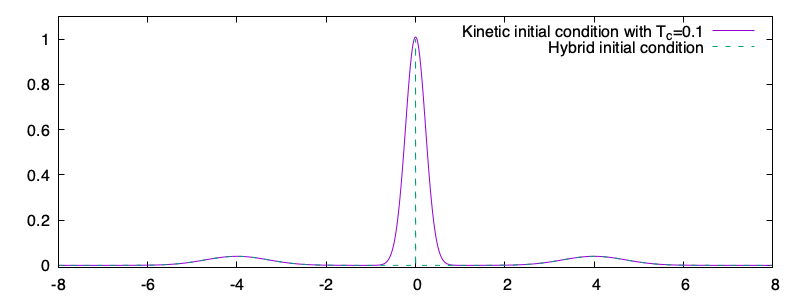
\includegraphics[width=0.8\textwidth]{img/distribution.png}
  \end{figure}

  \mbold{Goal:}
  \begin{itemize}
    \item Check numerically the validity of the hybrid model versus the full kinetic model of Vlasov-Poisson equations
  \end{itemize}
\end{frame}

\begin{frame}{Outline}
  \tableofcontents
\end{frame}

\section{Modelization}
%%%%%%%%%%%%%%%%%%%%%%%%%%%%%%%%%%%%%%%%%%%%%%%%%%%%%%%%%%%%%%%%%%%%%

\begin{frame}{Vlasov-Poisson-Ampère equations 1D$x$ $\times$ 1D$v$}
  Our model: transport of electron density distribution $f = f(t,x,v)$:
  $$
    \begin{cases}
      \partial_t f + v\partial_x f + E\partial_v f = 0 \\
      \partial_x E = \int_\mathbb{R} f\,\mathrm{d}v - 1 \\
      \partial_t E = -\int_{\mathbb{R}}vf\,\mathrm{d}v + \frac{1}{|\Omega|}\int_\Omega\int_\mathbb{R}vf\,\mathrm{d}v\mathrm{d}x
    \end{cases}\qquad(x,v)\in \Omega\times\mathbb{R}
  $$
  \mbold{Motivations:}
  \begin{itemize}
    \item We consider an initial condition of the form: $f = f_c + f_h$ with: $f_c(t=0,x,v) = \mathcal{M}_{\rho_c,u_c,T_c}(v) \underset{T_c\to 0}{=} \delta_{v-u_c}(v)\rho_c(t=0,x)$
    \item We want high order methods in $(x,v)$ \begin{itemize}\item FFT in $x$ + WENO in $v$\end{itemize}
    \item We want high order methods in time $t$ \begin{itemize}\item splitting method \emph{vs} exponential integrator\end{itemize}
  \end{itemize}
\end{frame}

\begin{frame}{The idea}
  \begin{itemize}
    \item Grid methods can't have an initial condition like : $f_0(x,v) = \rho_{c,0}(x){\color{red}\delta_{v-u_c}(v)} + f_{h,0}(x,v)$
    \item Idea is to derive an hybrid model : \begin{itemize}
      \item Cold plasma approximation: $\!\!\frac{T_c}{T_h}\! \ll\! 1$\ \arrow\ $f_c(t,x,v)\! =\! \rho_c(t,x)\delta_{v-u_c(t,x)}(\!v\!)$: \begin{itemize}
        \item Fluid dynamic for cold particles (no velocity grid)
      \end{itemize}
      \item Hypothesis on hot particles: $\int_\mathbb{R} f_h(t,x,v)\,\mathrm{d}v \ll \rho_c(t,x)$: \begin{itemize}
        \item Kinetic dynamic for hot particles
      \end{itemize}
    \end{itemize}
  \end{itemize}
\end{frame}

\begin{frame}{Derivation of hybrid model}
  $$
    \begin{cases}
      \int_\mathbb{R} \begin{pmatrix}1\\v\end{pmatrix} \Big( \partial_t f_c + v\partial_xf_c + E\partial_v f_c = 0 \Big)\,\mathrm{d}v \\
      \partial_t f_h + v\partial_xf_h + E\partial_vf_h = 0 \\
      \partial_x E = \int_\mathbb{R}f_c\,\mathrm{d}v + \int_\mathbb{R}f_h\,\mathrm{d}v - 1 \\
      \partial_t E = - \int_\mathbb{R}vf_c\,\mathrm{d}v - \int_\mathbb{R}vf_h\,\mathrm{d}v + \frac{1}{|\Omega|}\int_\Omega\int_\mathbb{R} v(f_c+f_h)\,\mathrm{d}v\mathrm{d}x
    \end{cases}
  $$
  we note: $$
    \begin{pmatrix}
      \rho_c(t,x)\\ \rho_c(t,x)u_c(t,x)
    \end{pmatrix} = \int_\mathbb{R}\begin{pmatrix}1\\v\end{pmatrix}f_c(t,x,v)\,\mathrm{d}v
  $$
  and \emph{cold plasma approximation}: $f_c(t,x,v) = \rho_c(t,x)\delta_{v=u_c(t,x)}(v)$
\end{frame}
\begin{frame}{Non-linear hybrid fluid-kinetic model}
  $$
    \begin{cases}
      \partial_t \rho_c + \partial_x(\rho_cu_c) = 0\\
      \partial_t(\rho_cu_c) + \partial_x(\rho_cu_c^2)-\rho_cE = 0\\
      \partial_tf_h + v\partial_xf_h + E\partial_vf_h = 0\\
      \partial_tE = -\rho_cu_c - \int_\mathbb{R}vf_h\,\mathrm{d}v + \frac{1}{|\Omega|}\left(\int_\Omega\int_\mathbb{R}vf_h\,\mathrm{d}v\mathrm{d}x + \int_\Omega\rho_cu_c\,\mathrm{d}x \right)\\
      {\color{red}\left(\phantom{\frac{}{}}\right.} \partial_xE = \rho_c + \int_\mathbb{R}f_h\,\mathrm{d}v - 1 {\color{red}\left.\phantom{\frac{}{}}\right)}
    \end{cases}
  $$
  \begin{itemize}
    \item If Poisson equation satisfied initially, the equation is propagated with time.
    %\item The initial condition $(u_c^0,f_h^0,E^0,\rho_c^0)$ satisfies Poisson equation \begin{itemize}
    %  \item $\partial_x E_0(x) = \rho_c^0(x) + \int_\mathbb{R}f_h^0(x,v)\,\mathrm{d}v$
    %\end{itemize}
    %\item We can compute cold density $\rho_c$ $\forall t\geq0$ with Poisson equation
    %\item In other words, we don't need to compute $\rho_c$ at each time
  \end{itemize}
  %Now we want an \emph{easy to compute} model, we linearize this non-linear model
  Following physicists framework, we linearize this non-linear model
\end{frame}

\begin{frame}{Linearization of hybrid fluid-kinetic model}
  Linearization near equilibrium :
  $$
    \begin{aligned}
      \rho_c(t,x)   =& \rho_c^{(0)}(x) & + & \varepsilon \rho_c^{(1)}(t,x) \\
         u_c(t,x)   =&                 &   & \varepsilon  u_c^{(1)}(t,x) \\
           E(t,x)   =&                 &   & \varepsilon  E^{(1)}(t,x) \\
         f_h(t,x,v) =& f_h^{(0)}(v)    & + & \varepsilon  f_h^{(1)}(t,x,v) \\
    \end{aligned}
  $$
  We obtain \mbold{Linear hybrid model} (LHM):
  $$
    \begin{cases}
      \partial_tu_c{\color{gris}^{(1)}}  = E{\color{gris}^{(1)}}  {\color{gris}+ \mathcal{O}(\varepsilon)} \\
      \partial_tE{\color{gris}^{(1)}}    = -\rho_c^{(0)}u_c{\color{gris}^{(1)}} - \int_\mathbb{R}vf_h{\color{gris}^{(1)}}\,\mathrm{d}v {\color{gris}+ \mathcal{O}(\varepsilon)}\\
      \partial_tf_h{\color{gris}^{(1)}}  + v\partial_xf_h{\color{gris}^{(1)}} + E\partial_vf_h{\color{gris}^{(1)}} = 0 {\color{gris}+ \mathcal{O}(\varepsilon)}
    \end{cases}
  $$
  \mbold{Properties:} conservation of mass and total energy \cmark

  All this derivation can be generalized to 3D$x$-3D$v$ \begin{thebibliography}{9}
    \setbeamertemplate{bibliography item}[article]
    \bibitem{a} \customcite{Holderied:2020}
  \end{thebibliography}
\end{frame}

\begin{frame}{Poisson bracket}
  LHM has an hamiltonian structure. The Poisson bracket is define by:
  $$
    \begin{aligned}
      \{ {\cal F}, {\cal G} \}( u, E, f) &= \int_{\mathbb{R}}\int_{\mathbb{R}} f \left( \partial_x \frac{\delta {\cal F}}{\delta f}\partial_{v} \frac{\delta {\cal G}}{\delta f} - \partial_{v} \frac{\delta {\cal F}}{\delta f}\partial_{x} \frac{\delta {\cal G}}{\delta f}\right)\mathrm{d}v \mathrm{d}x \\
                           & + \int_{\mathbb{R}}  \left(  \frac{\delta {\cal F}}{\delta{ u}}  \frac{\delta {\cal G}}{\delta{ E}} - \frac{\delta {\cal F}}{\delta{ E}}  \frac{\delta {\cal G}}{\delta{u}} \right) \mathrm{d}x \\
                           & + \int_{\mathbb{R}}\int_{\mathbb{R}}  \left(  \frac{\delta {\cal F}}{\delta{ E}}  \partial_v f\frac{\delta {\cal G}}{\delta{ f}} - \frac{\delta {\cal G}}{\delta{ E}} \partial_v f \frac{\delta {\cal F}}{\delta{f}} \right) \mathrm{d}{ v}\mathrm{d}x \\
    \end{aligned}
  $$
  and Hamiltonian by:
  $$
    \mathcal{H}(t) = \underbrace{\frac{1}{2}\int_\mathbb{R}E^2\,\mathrm{d}x}_{\mathcal{H}_{E}}
                   + \underbrace{\frac{1}{2}\int_\mathbb{R}\rho_c^{(0)}u_c^2\,\mathrm{d}x}_{\mathcal{H}_{u_c}}
                   + \underbrace{\frac{1}{2}\int_\Omega\int_\mathbb{R}v^2f_h\,\mathrm{d}v\mathrm{d}x}_{\mathcal{H}_{f_h}}
  $$
\end{frame}

\section{Numerical scheme}
%%%%%%%%%%%%%%%%%%%%%%%%%%%%%%%%%%%%%%%%%%%%%%%%%%%%%%%%%%%%%%%%%%%%%

\begin{frame}{Hamiltonian splitting}
  We would like to implement a splitting method inspired by a hamiltonian splitting.

  With $U=\begin{pmatrix}u_c\\E\\f_h\end{pmatrix}$ problem can be written as:
  $$
    \begin{aligned}
      \dot{U} &= \{U,\mathcal{H}\} \\
              &= \{U,\mathcal{H}_{E}\} + \{U,\mathcal{H}_{u_c}\} + \{U,\mathcal{H}_{f_h}\}
    \end{aligned}
  $$
  We obtain the splitting:
  \begin{itemize}
    \item $\dot{U} = \{U,\mathcal{H}_{E}\}$   \hfill \arrow \hfill solution is $\varphi^{[E]}_t(U^0)$
    \item $\dot{U} = \{U,\mathcal{H}_{u_c}\}$ \hfill \arrow \hfill solution is $\varphi^{[u_c]}_t(U^0)$
    \item $\dot{U} = \{U,\mathcal{H}_{f_h}\}$ \hfill \arrow \hfill solution is $\varphi^{[f_h]}_t(U^0)$
  \end{itemize}
  Hamiltonian structure paves the way of a splitting method.
\end{frame}


\subsection{Splitting method}
\begin{frame}{Splitting method}
  \begin{itemize}
    \item \mbold{Lie:} order 1 method, composition of substeps: $$U(t^{n+1})\approx U^{n+1} = \varphi^{[E]}_{\Delta t} \circ \varphi^{[u_c]}_{\Delta t} \circ \varphi^{[f_h]}_{\Delta t}(U^n)$$
    \item \mbold{Strang:} order 2 method, for a 3 steps formulation: $$U^{n+1} = S_{\Delta t}(U^n) = \varphi^{[f_h]}_{\Delta t/2} \circ \varphi^{[u_c]}_{\Delta t/2} \circ \varphi^{[E]}_{\Delta t} \circ \varphi^{[u_c]}_{\Delta t/2} \circ \varphi^{[f_h]}_{\Delta t/2} (U^n) $$ \begin{thebibliography}{9}
    \setbeamertemplate{bibliography item}[article]
    \bibitem{a} \customcite{Strang:1968}
  \end{thebibliography}
    \item \mbold{Suzuki:} order 4 method, composition of 5 Strang methods: $$
      U^{n+1} = \mathcal{S}_{\Delta t}(U^n) = S_{\alpha_1\Delta t} \circ S_{\alpha_2\Delta t} \circ S_{\alpha_3\Delta t} \circ S_{\alpha_2\Delta t} \circ S_{\alpha_1\Delta t} (U^n)
    $$with: $$ \alpha_1 = \alpha_2 = \frac{1}{4 - \sqrt[3]{4}} \qquad \alpha_3 = \frac{1}{1- 4^{\frac{2}{3}}}$$ \begin{thebibliography}{9}
    \setbeamertemplate{bibliography item}[article]
    \bibitem{a} \customcite{Suzuki:1990}
    \bibitem{a} \customcite{Casas:2020}
  \end{thebibliography}
  \end{itemize}
  % TODO other optimized methods split into 3 parts Casas et al.
\end{frame}
\begin{frame}{Numerical resolution of each step}
  \only<1>{
    $$
      \varphi^{[E]}(U) = \begin{cases}
        \partial_t u_c = E \\ \partial_t E = 0 \\ \partial_t f_h = -E\partial_vf_h
      \end{cases}
       \rightarrow 
      \varphi^{[E]}_{\Delta t}(U^n) = \begin{pmatrix}u_c^n + \Delta t E^n \\ E^n \\ f_h^n(x,v-\Delta t E^n)\end{pmatrix}
    $$
    \mbold{Numerical tools:}
    \begin{itemize}
      \item Lagrange 5 interpolation to approximate $f_h(x,v-\Delta t E^n)$
      \item More costly step, so we keep it in the middle of Strang method
    \end{itemize}
  }\only<2>{
    $$
      \varphi^{[u_c]}(U) = \begin{cases}
        \partial_t u_c = 0 \\ \partial_t E = -\rho_c^{(0)}u_c \\ \partial_t f_h = 0
      \end{cases}
       \rightarrow 
      \varphi^{[u_c]}_{\Delta t}(U^n) = \begin{pmatrix}u_c^n \\ E^n-\Delta t\rho_c^{(0)}u_c^n \\ f_h^n\end{pmatrix}
    $$
    \mbold{Numerical tools:}
    \begin{itemize}
      \item Fastest step
    \end{itemize}
  }\only<3>{
    $$
      \varphi^{[f_h]}(U) =\! \begin{cases}
        \partial_t u_c = 0 \\ \partial_t E = -\int_\mathbb{R}vf_h\,\mathrm{d}v \\ \partial_t f_h = -v\partial_xf_h
      \end{cases}\!\!\!\!\!\!
      \rightarrow
      \varphi^{[f_h]}_{\Delta t}(U^n)\!=\!\!\begin{pmatrix}u_c^n \\ \!\!\hat{E}^n - \frac{i}{k}\int_\mathbb{R}(e^{-ikv\Delta t}-1)\hat{f}_h^n\,\mathrm{d}v\!\! \\ e^{-ikv\Delta t}\hat{f}_h^n\end{pmatrix}
    $$
    \mbold{Numerical tools:}
    \begin{itemize}
      \item FFT and iFFT during this step
      \item Fast with \texttt{fftw} if you reuse allocated memory
    \end{itemize}
  }
\end{frame}

\subsection{Lawson method}
\begin{frame}{Lawson method}
  Fluid part is linear, we want to solve it exactly \arrow Lawson method
  $$
    \partial_t \underbrace{\begin{pmatrix}
      u_c\\E\\\hat{f}_h
    \end{pmatrix}}_{U} + \underbrace{\begin{pmatrix}
      0 & -1 & 0 \\ \rho_c^{(0)} & 0 & 0 \\ 0 & 0 & ikv
    \end{pmatrix}}_{A} \begin{pmatrix}
      u_c\\E\\\hat{f}_h
    \end{pmatrix} + \underbrace{\begin{pmatrix}
      0\\\int_\mathbb{R}vf_h\,\mathrm{d}v \\\widehat{E\partial_vf_h}
    \end{pmatrix}}_{F(U)} = 0
  $$
  We rewrite as:
  $$
    \partial_t\underbrace{\left(e^{tA}U\right)}_{V} + e^{tA}F(\underbrace{U}_{e^{-tA}V}) = 0
  $$
  and now we solve with a RK method: $\partial_tV = -e^{tA}F(e^{-tA}V)$ and next rewrite with the $U$ variable. For example with Lawson Euler method:
  $$
    V(t^n+\Delta t) \approx V^{n+1} = V^n - \Delta t e^{t^nA}F(e^{-t^nA}V^n)
  $$
  or as an expression of $U$:
  $$
    U^{n+1} = e^{-\Delta t A}U^n - \Delta te^{-\Delta t A}F(U^n)
  $$
  %\arrow\ $e^{tA}$ has an explicit form \cmark
\end{frame}

\begin{frame}{Space integrators with Lawson method}
  \mbold{Numerical tools:}
  \begin{itemize}
    \item FFT in $x$ direction
    \item WENO5 in $v$ direction to approximate $\widehat{E\partial_vf_h}$
  \end{itemize}

  \mbold{CFL:} Lawson(RK(4,4))--WENO5 : $\Delta t\leq\frac{\sigma}{\|E^n\|_\infty}$, with $\sigma=1.433$
  \begin{thebibliography}{9}
    \setbeamertemplate{bibliography item}[article]
    \bibitem{a} \customcite{Crouseilles:2019b}
  \end{thebibliography}
\end{frame}

\section{Adaptive time step methods}
%%%%%%%%%%%%%%%%%%%%%%%%%%%%%%%%%%%%%%%%%%%%%%%%%%%%%%%%%%%%%%%%%%%%%
\begin{frame}{Main idea of adaptive time step methods (error estimate)}
  For a generic ODE $\dot{u} = f(t,u(t))$, adaptive time step method needs 2 numerical estimations of solution $u(t^{n+1})$ of different order, $p$ and $p+1$:
  $$
    u^{n+1}_{[p]} = u(t^{n+1}) + \mathcal{O}\left(\Delta t^{p+1}\right)
    \qquad
    u^{n+1}_{[p+1]} = u(t^{n+1}) + \mathcal{O}\left(\Delta t^{p+2}\right)
  $$
  Estimate of the local error:
  $$
    L^{n+1}_{[p]} = \left| u^{n+1}_{[p+1]} - u^{n+1}_{[p]} \right|
  $$
  If $L^{n+1}_{[p]} > \text{tol}$: we reject the step and  start again from time $t^n$. Else we accept the step. In both cases, the optimal new time step is:
  $$
    \Delta t_\text{opt} = \sqrt[p]{\frac{\text{tol}}{ L^{n+1}_{[p]}}}\Delta t^n
  $$
  In practice we don't want volatile time step: $\Delta t^{n+1} = \max\left(0.5\Delta t^n,\min\left(2\Delta t^n,\Delta t_\text{opt}\right)\right)$
\end{frame}

\subsection{Splitting method}
\begin{frame}{Adaptive time step method for splitting method}
  For the Suzuki splitting method:
  \begin{thebibliography}{9}
    \setbeamertemplate{bibliography item}[article]
    \bibitem{a} \customcite{Blanes:2019}
  \end{thebibliography}
  $$
    U^{n+1}_{[4]} = \mathcal{S}_{\Delta t}(U^n)
      = S_{\alpha_1\Delta t}
        \circ \underbrace{ S_{\alpha_2\Delta t}
        \circ \underbrace{ S_{\alpha_3\Delta t}
        \circ \underbrace{ S_{\alpha_2\Delta t}
        \circ \underbrace{ S_{\alpha_1\Delta t} (U^n). }_{U^{(1)}}
                                                      }_{U^{(2)}}
                                                      }_{U^{(3)}}
                                                      }_{U^{(4)}}
  $$
  We compute an order 3 approximation from $U^n$ and $U^{(s)}$, $s=1,2,3,4$ :
  $$
    U^{n+1}_{[3]} = -U^n + w_1(U^{(1)}+U^{(4)}) + w_2(U^{(2)}+U^{(3)})
  $$
  with:
  $$
    w_1 = \frac{g_2(1-g_2)}{g_1(g_1-1)-g_2(g_2-1)},\quad w_2 = 1-w_1, \quad \begin{aligned}g_1 &= \alpha_1\\ g_2&=\alpha_1+\alpha_2\end{aligned}
  $$
  and $L^{n}_{[3]} = \left\| U^{n+1}_{[4]} - U^{n+1}_{[3]} \right\|_2$
\end{frame}


\subsection{Lawson method}
\begin{frame}{Adaptive time step method for Lawson method}
  Lawson methods are built on Runge-Kutta method, embedded Lawson method are written with an underlying embedded Runge-Kutta method.

  \begin{thebibliography}{9}
    \setbeamertemplate{bibliography item}[article]
    \bibitem{a} \customcite{Dormand:1978}
  \end{thebibliography}
  With DP4(3) (Dormand-Prince method of order 4, with embedded 3 method):
  \[
    \begin{array}{c|cccccc}
      0           &             &             &             &             &                & \multirow{5}{*}{\left.\phantom{\begin{matrix}0\\1\\2\\3\\4\end{matrix}}\right\}\text{Classical RK(4,4)}} \\
      \frac{1}{2} & \frac{1}{2} &             &             &             &                & \\
      \frac{1}{2} & 0           & \frac{1}{2} &             &             &                & \\
      1           & 0           & 0           & 1           &             &                & \\
    \cline{1-6}
      1           & \frac{1}{6} & \frac{1}{3} & \frac{1}{3} & \frac{1}{6} &                &\\
    \cline{1-6}
                  & \frac{1}{6} & \frac{1}{3} & \frac{1}{3} & \frac{2}{30} & \frac{1}{10}  & 
    \end{array}
  \]
            %\left.\phantom{ \begin{pmatrix}1\\2\\3\\4\\5 \end{pmatrix}}\right\)
  We compute a 3\textsuperscript{rd} order approximation from $U^n$, $U^{(s)}$, $s=1,2,3,4$ done by the last line of Butcher tableau.

  And $L^{n}_{[3]} = \left\| U^{n+1}_{[4]} - U^{n+1}_{[3]} \right\|_2$
\end{frame}

\section{Relation of dispersion}
%%%%%%%%%%%%%%%%%%%%%%%%%%%%%%%%%%%%%%%%%%%%%%%%%%%%%%%%%%%%%%%%%%%%%
\begin{frame}{Sketch of computing}
  We linearize around unstable equilibrium state (TSI type):
  \begin{itemize}
    \item for kinetic model $$f_\text{eq}(v) = \mathcal{M}_{1-\alpha,0,{\color{red}T_c}}(v) + \mathcal{M}_{^\alpha/_2,v_0,1}(v) + \mathcal{M}_{^\alpha/_2,-v_0,1}(v)$$
    \item for LHM $$
      \begin{aligned}
        U_\text{eq} &= \left(u_{c,\text{eq}},E_\text{eq},f_{h,\text{eq}}\right)^\text{T} \\
                    &= \left(0,0, \mathcal{M}_{^\alpha/_2,v_0,1} + \mathcal{M}_{^\alpha/_2,-v_0,1}\right)^\text{T}
      \end{aligned}
    $$
  \end{itemize}

  We obtain 2 relations of dispersion:
  \begin{itemize}
    \item One for kinetic model, depends on $T_c$: $D^K_{[T_c]}(k,\omega)$
    \item One for linear hybrid model (LHM): $D^{LHM}(k,\omega)$
  \end{itemize}
\end{frame}

\begin{frame}{Relations of dispersion}
  \begin{itemize}
    \item \mbold{Kinetic model:}$$\begin{aligned}
    \!\!\!\!\!\!\!\!\!\!\!\!\!\!\!D^K_{[T_c]}(k,\omega) = 1 - \frac{1}{k^2}\left[\vphantom{\frac{}{\sqrt{}}}\right. & -\frac{1-\alpha}{T_c}\left( 1 + \frac{1}{\sqrt{2T_c}}\frac{\omega}{k}Z\left( \frac{1}{\sqrt{2T_c}}\frac{\omega}{k}\right) \right) \\
                                          & {\color{violet}-\frac{\alpha}{2}\left( 1 + \frac{1}{\sqrt{2}}\left(\frac{\omega}{k}-v_0\right)Z\left(\!\!\frac{1}{\sqrt{2}}\!\!\left(\frac{\omega}{k}-v_0\right)\right) \right)} \\
                                          & \left. {\color{bleu}-\frac{\alpha}{2}\left( 1 + \frac{1}{\sqrt{2}}\left(\frac{\omega}{k}+v_0\right)Z\left(\!\!\frac{1}{\sqrt{2}}\!\!\left(\frac{\omega}{k}+v_0\right)\right) \right)}  \right]
  \end{aligned}$$
  \item \mbold{LHM:}$$
  \begin{aligned}
      \!\!\!\!\!\!\!\!\!\!\!\!\!\!\!D^{LHM}(k,\omega)
    &=1-\frac{1}{k^2}\left[\left(1-\alpha\right)\frac{k^2}{\omega^2}{\color{violet}-\frac{\alpha}{2}\left(1+\frac{1}{\sqrt{2}}\left(\frac{\omega}{k}-v_0\right)Z\left(\!\!\frac{1}{\sqrt{2}}\!\!\left(\frac{\omega}{k}-v_0\right)\right)\right)}\right.\nonumber\\
    &~~~~~~~~~~~~~~~\left.{\color{bleu}-\frac{\alpha}{2}\left(1+\frac{1}{\sqrt{2}}\left(\frac{\omega}{k}+v_0\right)Z\left(\!\!\frac{1}{\sqrt{2}}\!\!\left(\frac{\omega}{k}+v_0\right)\right)\right)}\right]
  \end{aligned}
  $$
  \end{itemize}
  where $Z(z) = \sqrt{\pi}e^{-z^2}(i-\erfi(z))$ (Fried and Conte function)
\end{frame}

\begin{frame}{Convergence of relations of dispersion}

  Since $$Z(z) \underset{z\to+\infty}{\sim} -\frac{1}{z} - \frac{1}{2z^3} - \frac{3}{4z^5} + \mathcal{O}(z^{-7})$$
  with $z = \frac{1}{\sqrt{2T_c}}\frac{\omega}{k}$ when $T_c\to 0$ we get:
  $$
    -\frac{1-\alpha}{T_c}\left(\!1+\frac{1}{\sqrt{2T_c}}\frac{\omega}{k}Z\left(\frac{1}{\sqrt{2T_c}}\frac{\omega}{k}\right)\!\right)
    =
    -\frac{1-\alpha}{T_c}\left(\!- \frac{1}{2\left(\frac{1}{\sqrt{2T_c}}\frac{\omega}{k}\right)} + \mathcal{O}(z^{-4})\!\right)
  $$
  which is equivalent to:
  $$
    \frac{1-\alpha}{T_c}\frac{k^2T_c}{\omega^2} = (1-\alpha)\frac{k^2}{\omega^2}
  $$

  We have: $$\lim_{T_c\to 0}D^K_{[T_c]}(k,\omega) = D^{LHM}(k,\omega)\quad\text{\cmark}$$
\end{frame}

\begin{frame}{Slope of both relations of dispersion}
  \begin{figure}\centering
    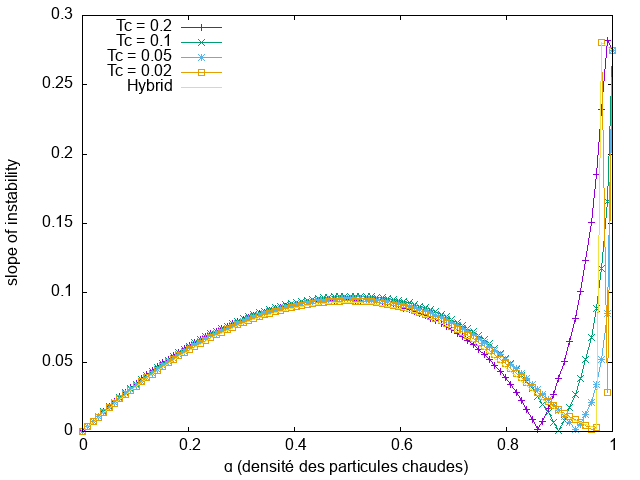
\includegraphics[height=0.8\textheight]{img/limit_slope_alpha.png}
  \end{figure}
\end{frame}

\section{Numerical results}
%%%%%%%%%%%%%%%%%%%%%%%%%%%%%%%%%%%%%%%%%%%%%%%%%%%%%%%%%%%%%%%%%%%%%

\begin{frame}{Validation of hybrid model}
  $\alpha = 0.2$,$\epsilon=10^{-2}$, $k=0.5$, $x\in[0,\frac{2\pi}{k}]$, $v\in[-12,12]$, $v_0 = 4$ \\
  $N_x = 135$, $N_v = 1200, $, $\Delta t = 0.5\Delta v$ for kinetic and LHM
  \only<1>{
    \begin{figure}\centering
      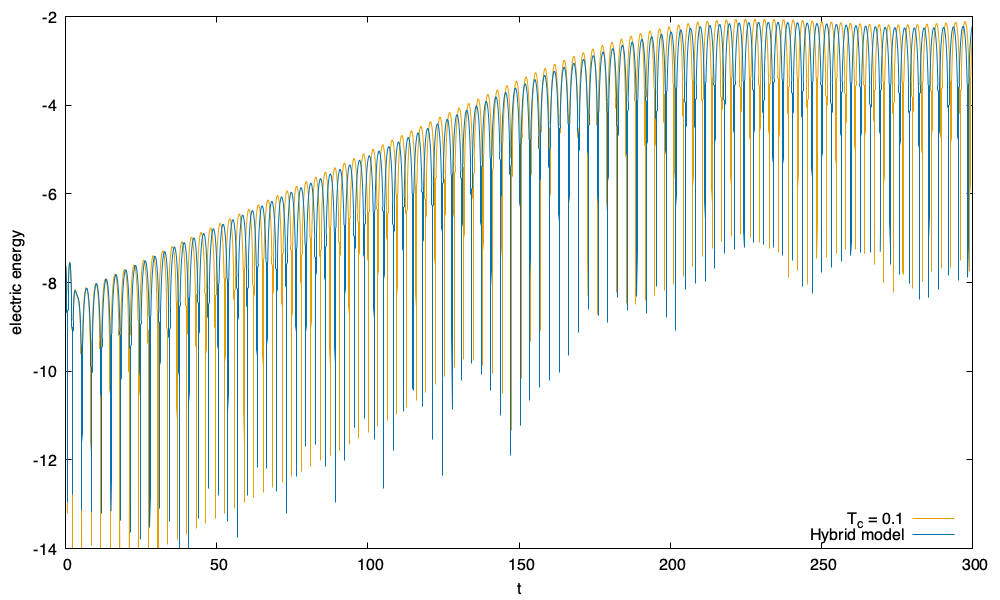
\includegraphics[width=0.8\textwidth]{img/limit_ee_Tf300.png}
    \end{figure}
  }\only<2>{
    \begin{figure}\centering
      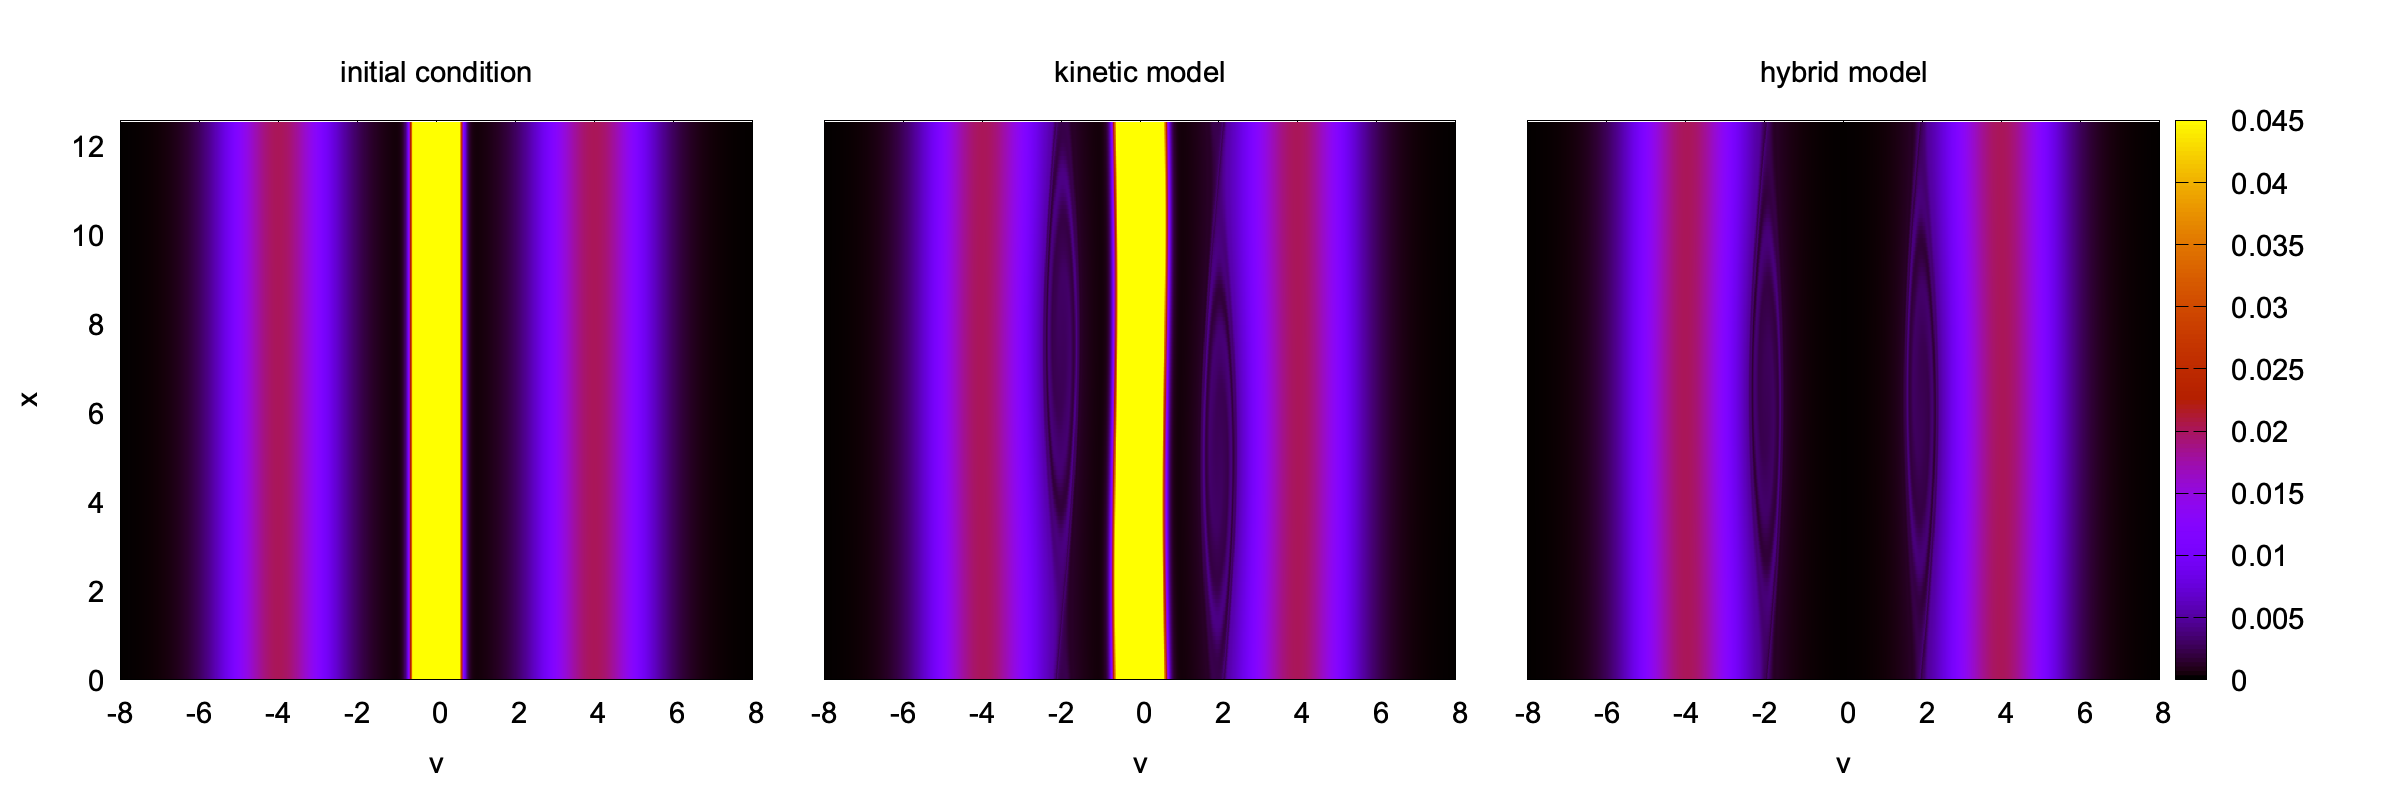
\includegraphics[width=\textwidth]{img/limit_vp.png}
    \end{figure}
  }
\end{frame}

\begin{frame}{Validation with relations of dispersion}
  Relations of dispersion give the electric energy approximation in the linear phase

  Perturbation $\epsilon=10^{-4}$, $\alpha=0.1$, $N_x = 135$, $N_v = 512$, $\Delta t = 0.5\Delta v$
  \only<1>{
    \begin{figure}\centering
      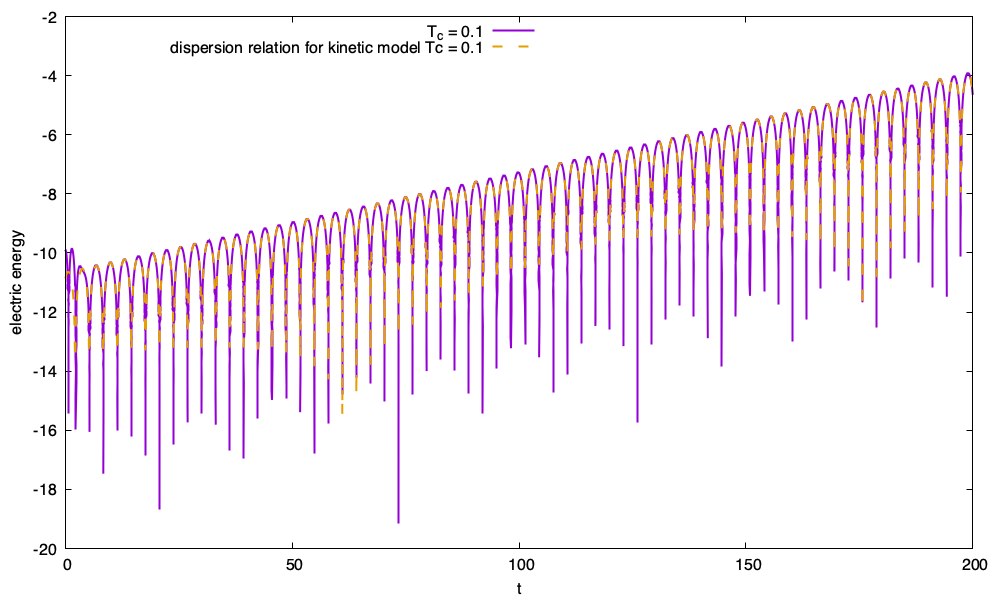
\includegraphics[width=0.8\textwidth]{img/limit_ee_Tf200_eps10m4.png}
    \end{figure}
  }\only<2>{
    \begin{figure}\centering
      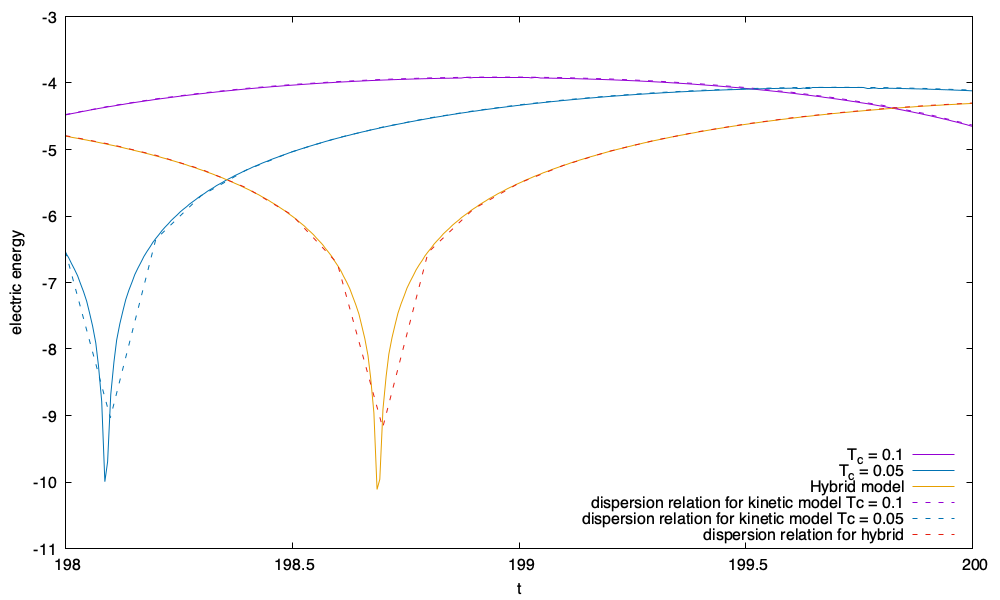
\includegraphics[height=0.75\textheight]{img/limit_ee_Tf200_cmp_zoom.png}
    \end{figure}
  }
\end{frame}

\begin{frame}{Convergence of kinetic model to linear hybrid model}
  $\alpha = 0.1$, $v\in[-12,12]$ \\
  $N_x = 135$, $N_v = 715, 764, 826, 1131$, $\Delta t = 0.5\Delta v$ for kinetic with $T_c = 0.2, 0.175, 0.15, 0.08$

  $N_v = 256$ for LHM
  \begin{columns}
    \begin{column}{0.5\textwidth}
      \begin{figure}\centering
        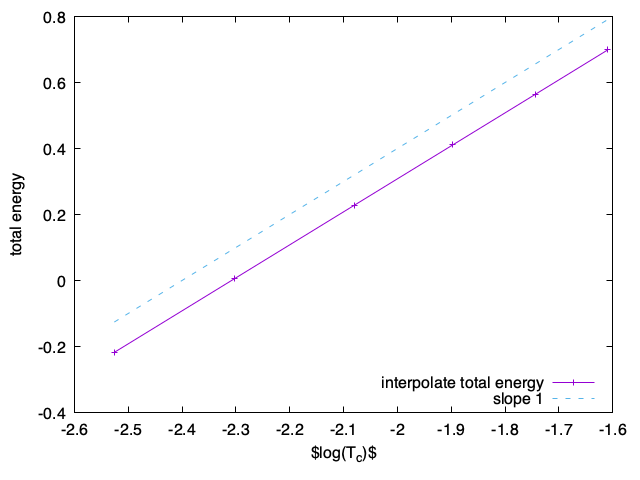
\includegraphics[width=\textwidth]{img/limit_slope_totalenergy.png}
      \end{figure}
    \end{column}
    \begin{column}{0.5\textwidth}
      \begin{figure}\centering
        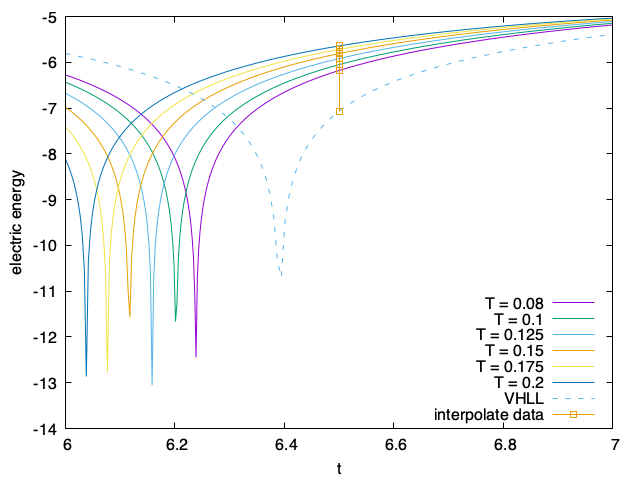
\includegraphics[width=\textwidth]{img/limit_ee.png}
      \end{figure}
    \end{column}
  \end{columns}
\end{frame}

\begin{frame}{Test adaptive time step method}
  $N_x = 81$, $N_v = 128$

  $\text{tol}=2\cdot10^{-4}$, $L = \| U^{n+1}_{[4]} - U^{n+1}_{[3]} \|_2$ is the local error
  \only<1>{
    \begin{figure}\centering
      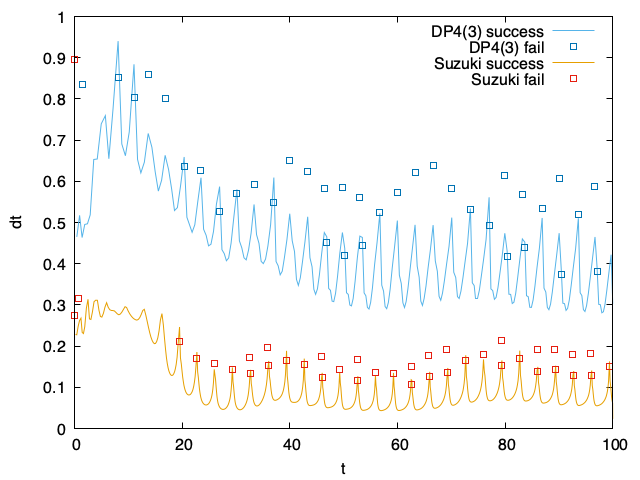
\includegraphics[width=0.8\textwidth]{img/compare_dt.png}
    \end{figure}
  }\only<2>{
    \begin{figure}\centering
      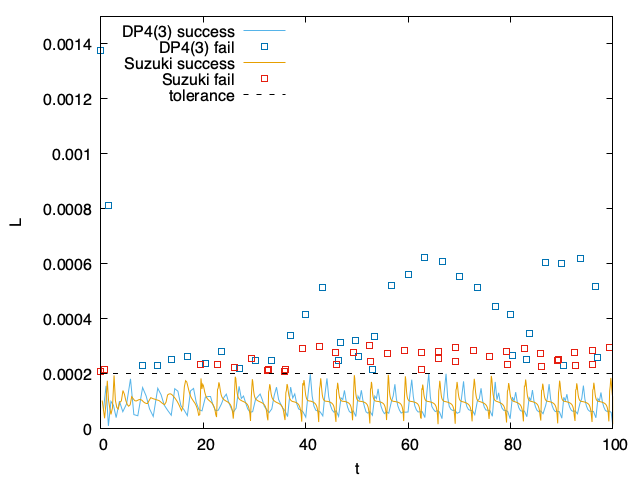
\includegraphics[width=0.8\textwidth]{img/compare_error_dtt.png}
    \end{figure}
  }
\end{frame}


\section{Conclusion}
%%%%%%%%%%%%%%%%%%%%%%%%%%%%%%%%%%%%%%%%%%%%%%%%%%%%%%%%%%%%%%%%%%%%%

\begin{frame}{Conclusion}
  \mbold{Summary}
  \begin{itemize}
    \item Validation and robustness of Linear Hybrid Model
    \item Derivation of geometric structure for LHM
    \item Numerical cost for one Strang is equivalent of one stage of Lawson-RK method \begin{itemize}
        \item 5 Strang for Suzuki
        \item 4 stages for RK(4,4)
      \end{itemize}
  \end{itemize}

  \mbold{Future works}
  \begin{itemize}
    \item Extension to 1D$x$ -- 3D$v$, same framework of {\color{PLB}\customcite{Holderied:2020}}\begin{itemize}
      \item Splitting into 6 sub-steps \arrow Strang in 11 steps
      \item Lawson methods should be more efficient
      \item Compare with PIC method
    \end{itemize}
  \end{itemize}
\end{frame}

\begin{frame}[t]
  First results with splitting method for 1D$x$ -- 3D$v$
  \begin{figure}\centering
    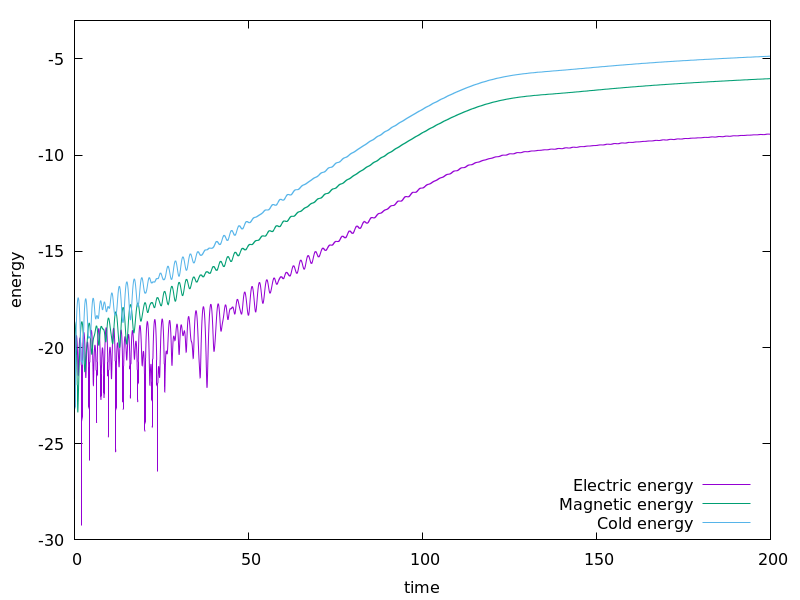
\includegraphics[height=0.8\textheight]{img/energy3dv.png}
  \end{figure}
  For Lawson method, I work on code generator from \texttt{sympy} expressions
\end{frame}

\begin{frame}[t]
  \vfill
  {\usebeamerfont{title} Thank you for your attention}
  \vfill
\end{frame}

\appendix
\backupbegin

\begin{frame}[plain]
  \vspace{0.65\textwidth}
  \hfill\footnotesize{Backup}
\end{frame}
%-------%
\begin{frame}{CPU time comparaison}
  \begin{figure}\centering
    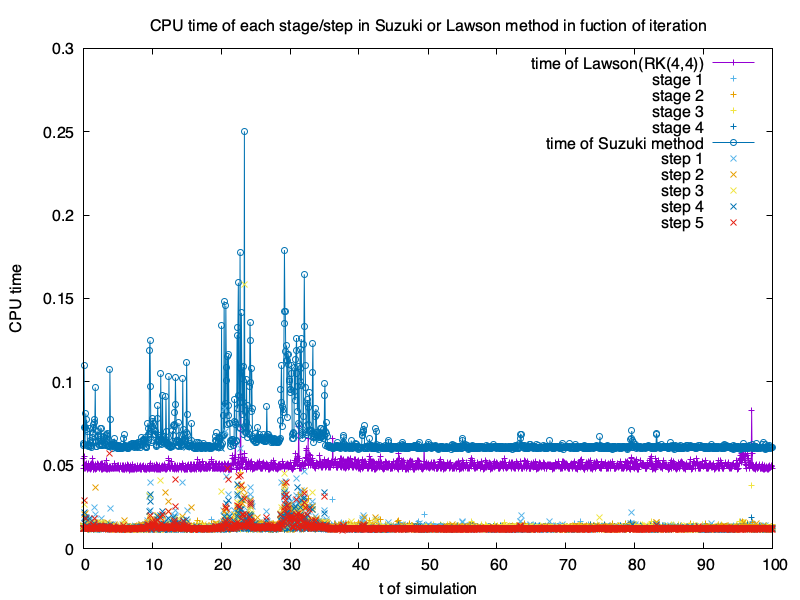
\includegraphics[height=0.8\textheight]{img/cputime.png}
  \end{figure}
\end{frame}


%-------%
\backupend

\end{document}

